\section{Sprzętowy System Archiwizacji}
    \subsection{Wybór Nośników (Dyski)}

    


    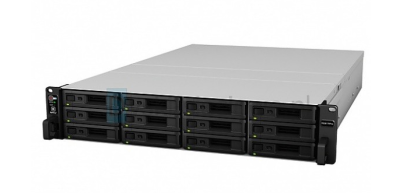
\includegraphics[width=0.3\textwidth]{nas.png}\\
        \textbf{Dyski NAS Synology RS3617RPxs}\\
       
        \begin{itemize}
            \item \textbf{Pojemność:} Skalowalne do 36 dysków, co pozwala na znaczne zwiększenie pojemności.
            \item \textbf{Prędkość Transferu:} Gigabit Ethernet i obsługa wielu interfejsów.
            \item \textbf{Redundancja:} Wsparcie dla RAID 0, 1, 5, 6, 10, F1.
        \end{itemize}


        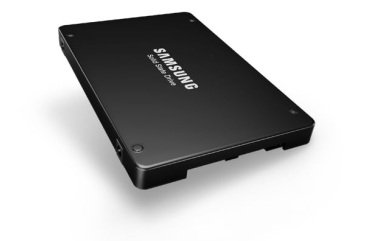
\includegraphics[width=0.3\textwidth]{spe.png}\\
        \textbf{Enterprise SSD Samsung PM1733}\\

        
        \begin{itemize}
            \item \textbf{Pojemność:} Wysoka pojemność i szybkość dostępu, idealne dla dużych baz danych.
            \item \textbf{Prędkość Transferu:} Bardzo wysoka prędkość odczytu i zapisu.
            \item \textbf{Redundancja:} Wykorzystanie w systemach RAID.
        \end{itemize}




    \subsection{Specyfikacja Techniczna Systemu Archiwizacji}

            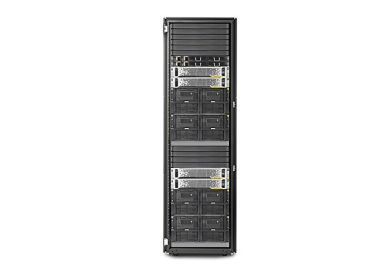
\includegraphics[width=0.3\textwidth]{hpe.png}\\
            \textbf{HPE StoreOnce 6500}\\


            \begin{itemize}
                \item \textbf{Architektura Systemu:} Duplikacja danych w celu optymalizacji miejsca i przepustowości.
                \item \textbf{Przepustowość:} Do kilku petabajtów pojemności w jednym systemie.
                \item \textbf{Zintegrowane Oprogramowanie:} Catalyst dla efektywnej replikacji danych.
            \end{itemize}

    \subsection{Zabezpieczenia Przed Utratą Danych}

            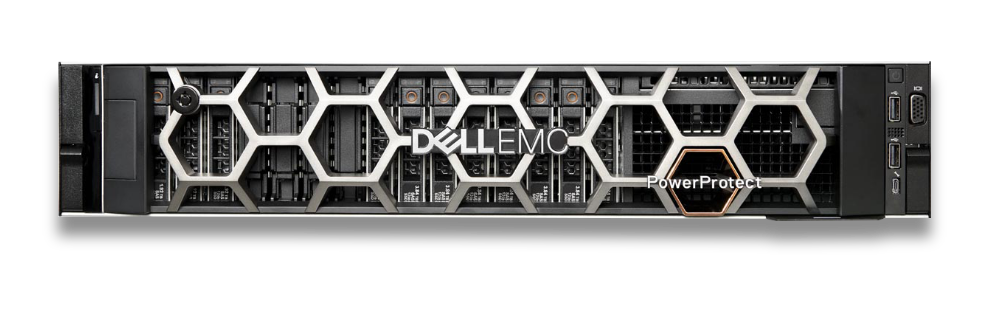
\includegraphics[width=0.3\textwidth]{del.png}\\
            \textbf{Dell EMC PowerProtect DD9900}\\
            \begin{itemize}
                \item \textbf{Kopie Bezpieczeństwa:} Skalowalne rozwiązanie do tworzenia kopii bezpieczeństwa.
                \item \textbf{Szyfrowanie:} Wbudowane funkcje szyfrowania danych.
                \item \textbf{Redundancja:} Automatyczne kopiowanie danych między różnymi lokalizacjami.
            \end{itemize}

    \subsection{Kosztorys Implementacji Systemu Archiwizacji}
    \begin{flushleft}
        \begin{table}[h]
            \renewcommand{\arraystretch}{1.5}
            \begin{tabular}{|l|l|}
                \hline
                \textbf{Nazwa} & \textbf{Cena (zł)} \\
                \hline
                Dyski NAS Synology RS3617RPxs & 16 551,00 \\
                Enterprise SSD Samsung PM1733 & 3 324,28 \\
                HPE StoreOnce 6500 & 1 334 576,59 \\
                Dell EMC PowerProtect DD9900 & Wycena indywidualna \\
                \hline
                \textbf{Suma} & \textbf{1 354 451,87} \\
                \hline
            \end{tabular}
        \end{table}
    \end{flushleft}



